\subsection{The basic situation of the participants}

The first aim of this study was to show how air pollution affected people’s daily activities by talking about the difference of college students’ activity in Tsinghua University. First let's saw part one of the questionnare, which surveyed participants’ basic situation. The situation of participants was listed in Table 1. It could be seen that the number of people in various professions was even. Most of the participants were grade 1 or grade 2 (85.3\%). The next question was sports frequency. As shown in the questionnare, many people did sports once or twice a week (47.1\%), then 32.4\% people did sports three to five times a week. The data showed that the students had a moderate amount of exercise. As for wearing masks, nearly sixty percent of participants sometimes wear masks during polluted day, about twenty percent of people always wear masks. We could also know that 67.6\% participants had their own air purifiers in their dormitorys. According to the first part of questionnare, it was obvious that most people had the consciousness to protect themselves in polluted air.

\begin{table}
\centering
\caption{Participants.}
\begin{tabular}{c|c|c}
Major & No. of Participants & Percentage of All Participants\\\hline
Education & 10 & 29.4\% \\
Literature & 13 & 8.8\% \\
Science & 4 & 11.8\% \\
Engineering & 14 & 41.2\% \\
Medicine & 3 & 8.8\%

\end{tabular}
\end{table}

\subsection{The maximum AQI value that participants could accept}
The second part of the questionnaire was the core content of this survey. We have selected eight different activities. Participants were supposed to indicate the maximum AQI value that they could accept for participating in these activities. The range of options in the questionnaire was 0~200. It could be considered that the data satisfied the truncated normal distribution with an interval of [0,200]. For each activity, the maximum likelihood estimation was used to find the mean and variance of the corresponding normal distribution. The probability density function for the truncated normal distribution was
$$p(x) = \frac{
    \frac{1}{\sqrt{2\pi}\sigma} e^{-\frac{(x-a)^2}{2\sigma^2}}
}{
    \int_0^{200} \frac{1}{\sqrt{2\pi}\sigma} e^{-\frac{(t-a)^2}{2\sigma^2}} dt
}$$
and the likelihood function was
$$lik(a,\sigma) = \frac{
    \frac{1}{(2\pi)^{\frac{n}{2}}\sigma ^n} e^{-\frac{1}{2\sigma^2}\sum_{i=1}^n(x_i-a)^2}
}{
    (\int_0^{200} \frac{1}{\sqrt{2\pi}\sigma} e^{-\frac{(t-a)^2}{2\sigma^2}} dt)^n
}$$
where $x_i, 1\leq i\leq n$ mean the data we got from questionnares.

The figure of the likelihood function was drawn in Matlab. We could find the initial point, which was used to calculate the maximun of the likelihood function, from the figure. And then the minimum point of the likelihood function was obtained by the Newton method. Taking the event "into the classroom" as an example, the image of the likelihood function was shown in Fig. 1. Select the initial point $(40,100)$, we could find the minimum point $(36.9,89.0)$. In other words, the mean value of the highest AQI that participants could accept in the classroom was $89.0$ , and the variance was $36.9$.

\begin{figure}
\centering
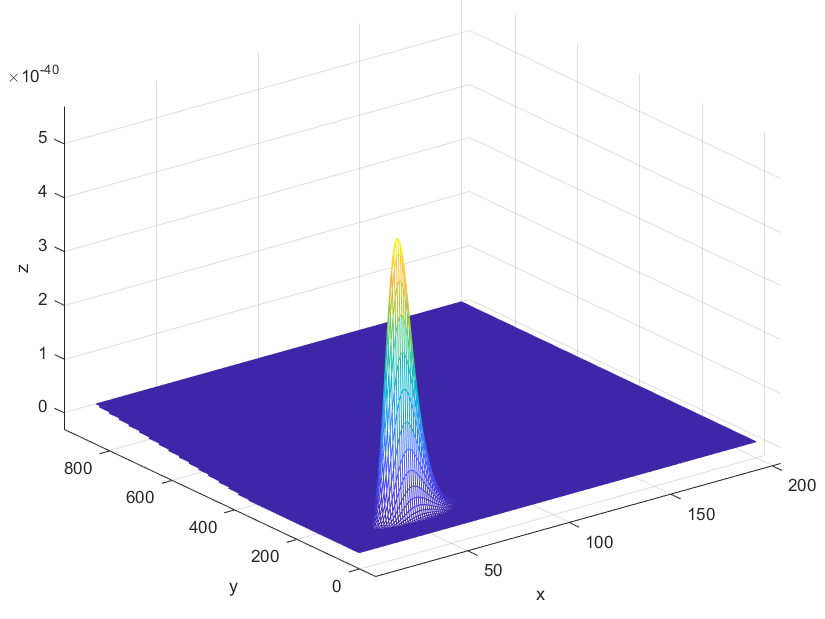
\includegraphics[width=0.8\textwidth]{1.png}
\caption{\label{fig:frog}Likelihood function about event "into the classroom".}
\end{figure}

The above operations were performed on all eight activities and the average and variance of the highest AQI values that the participants were able to accept under different activities were shown in Table 2. From Table 2 we could see that study in dormitory could accept the highest level of air pollution (115.5). On the contrary, some intense sports were most sensitive to air quality (72.7). Contrasting between the eight activities, the highest acceptable AQI for each activity was distributed around 100. The variances were distributed in range 30~50, so participants had about the same degree of dispersion of AQIs for the eight activities.

\begin{table}
\centering
\caption{The highest AQI values that the participants were able to accept under different activities.}
\begin{tabular}{c|c|c}
Activity & mean AQI & variance \\
\hline
go to class in classroom & 89.0 & 36.9 \\
study at library & 98.8 & 47.1 \\
go to PE class & 95.8 & 39 \\
some relaxing outside sports (walk, ride .etc) & 88.3 & 34.4 \\
some intense sports (football, basketball .etc) & 72.7 & 42.6 \\
meet classmates outside & 85.6 & 44.1 \\
run outside & 84.3 & 48.1 \\
study in dormitory & 115.5 & 45.8

\end{tabular}
\end{table}

\section{Discussion}

In this study, we studied the highest AQI value that everyone could accept under the eight activities. According to life experience, the amount of exercise capacity in the dormitory is small, so it should be the highest acceptable AQI value. Seeing the result, we found that the mean value of the study in dormitory was really the highest. Also, the low highest acceptable AQI value suggests that, the same to the hypothesis, it has great difference of college students’ activity between clean air and polluted air. This conclusion is most obvious for intense outdoor sports. Similar to other studies done before, this study illustrates the negative effects of air pollution from another perspective.

If people's highest accepted AQI meets the normal distribution in results part, then the percentage of people participating in the corresponding activities under different AQIs can be calculated, it is shown in Table 3. Pope (2002) suggested that Long-term exposure to combustion-related fine particulate air pollution is an important environmental risk factor for cardiopulmonary and lung cancer mortality. This has provided a theoretical basis for people to go out less in the polluted air.

\begin{table}
\centering
\caption{The percentage of people participating in the corresponding activities under different AQIs.}
\begin{tabular}{c|c|c|c|c|c|c|c|c}
AQI & class & lib & PE & sports(relax) & sports(intense) & meet & run & dormitory \\
\hline
20 & 0.969 & 0.953 & 0.974 & 0.976 & 0.892 & 0.932 & 0.909 & 0.981 \\
40 & 0.908 & 0.894 & 0.924 & 0.920 & 0.779 & 0.849 & 0.821 & 0.950 \\
60 & 0.784 & 0.795 & 0.821 & 0.795 & 0.617 & 0.719 & 0.693 & 0.887 \\
80&0.596 & 0.655 & 0.657 & 0.595 & 0.432 & 0.551 & 0.536 & 0.781 \\
100&0.383 & 0.490 & 0.457 & 0.367 & 0.261 & 0.372 & 0.372 & 0.632 \\
120&0.200 & 0.326 & 0.267 & 0.178 & 0.133 & 0.218 & 0.229 & 0.461 \\
140&0.083 & 0.191 & 0.129 & 0.066 & 0.057 & 0.109 & 0.123 & 0.296 \\
160&0.027 & 0.097 & 0.050 & 0.019 & 0.020 & 0.046 & 0.058 & 0.166 \\
180&0.007 & 0.042 & 0.015 & 0.004 & 0.006 & 0.016 & 0.023 & 0.080

\end{tabular}
\end{table}


We intend to further study how to take measures to reduce the impact of air pollution on people's activities and how to quantify the effectiveness of these measures. For example, change outdoor sports to indoor sports or install an air purifier. We hope that the follow-up study will help people reduce the impact of air pollution.
